\documentclass[a4paper,10pt]{article}

\usepackage[margin=1in]{geometry}
\usepackage{amsmath,amsthm,amssymb,hyperref}
%% For subfigure
\usepackage{caption,subcaption,graphicx}

\hypersetup{colorlinks=true,urlcolor=blue}

\usepackage{embedfile,fancyvrb}
\embedfile{\jobname.tex}

\usepackage{fancyhdr}
\pagestyle{fancy}
\lhead{Danny Hermes}
\rhead{Brad Poopy Head}

\renewcommand{\headrulewidth}{0pt}

\begin{document}

\textbf{NOTE:} To extract the \LaTeX\ source of this PDF and the supporting
files, execute:
\begin{Verbatim}[commandchars=\\\{\}]
pdftk \jobname.pdf unpack_files output .
\end{Verbatim}

We want to parameterize the three shapes so we can easily understand
what is happening. We assume the top of the sphere is \(0.3 \mu m\) away
from the horizontal cylinder, the sphere has a radius of \(0.1 \mu m\), the
vertical cylinder (dendrite) has diameter \(0.1 \mu m\) and the ``main line''
horizontal cylinder (that all the dendrites come out of has a diameter) of
\(1.0 \mu m\). We can visualize a cross-section of the top part via
\begin{verbatim}
H = 0.5;
theta = 0:0.01:(2*pi);
sphereIn2D = [0.1*cos(theta); 0.1*sin(theta) + 0.2 + H];

vertY = H:0.001:(H + 0.15);
leftPoints = [-0.05 * ones(size(vertY)); vertY];
rightPoints = [0.05 * ones(size(vertY)); vertY];
verticalCylinder = [leftPoints, rightPoints];

horizontalX = -0.3:0.001:0.3;
horizontalCylinder = [horizontalX; H * ones(size(horizontalX))];

allPoints = [sphereIn2D, verticalCylinder, horizontalCylinder];
scatter(allPoints(1, :), allPoints(2, :));
axis equal;

axis([-0.5, 0.5, 0.3, 1])
\end{verbatim}

\begin{figure}
  \centering
    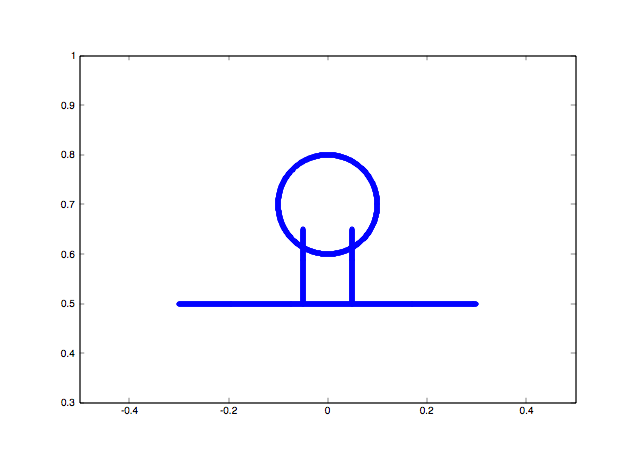
\includegraphics[scale=0.3]{cross_section.png}
  \caption{Cross-Section of Dendrite}
  \label{fig:1a}
\end{figure}

and see in Figure~\ref{fig:1a} the general cross-sectional geometry.

We need to find intersection points, but first get a basic idea of
the equations describing them:
\begin{itemize}
\item Top-Sphere: \(x^2 + y^2 + \left(z - 0.7\right)^2 = 0.1^2\). This has
a diameter of \(0.2 \mu m\) and has to be \(0.3 \mu m\) above the main
(horizontal) cylinder which is already \(0.5 \mu m\) above \(z = 0\), hence
we assume the center lies at \((0, 0, 0.5 + 0.3 - 0.1)
= (0, 0, 0.7)\) (since the radius is \(0.1\)).
\item Vertical Cylinder: \(x^2 + y^2 = \left(\frac{0.1}{2}\right)^2 =
0.05^2\). This is simply a circle of diameter \(0.1\) that extends infinitely
in the \(z\)-direction. This is assumed to be centered around \((x, y)
= (0, 0)\) but may change the \(x\) position of the center as we consider
dendrites on the left and/or right.
\item Horizontal Cylinder: \(y^2 + z^2 = \left(\frac{1.0}{2}\right)^2 =
0.5^2\). This is simply a circle of diameter \(0.1\) that extends infinitely
in the \(x\)-direction. This is the ``main line'' that all dendrites
sprout out of.
\end{itemize}

\textbf{Intersection points}: To find places where our geometries intersect
we need to find simultaneous solutions to the equations defining the
surfaces. For the intersection of the sphere and the dendrite cylinder,
we have
\[0.1^2 = x^2 + y^2 + \left(z - 0.7\right)^2 = 0.05^2 + \left(z -
0.7\right)^2.\]
This gives us
\[\left(z - 0.7\right)^2 = 0.0075 \Rightarrow z = 0.7 \pm \sqrt{0.0075}.\]
However, the top one of these points corresponds to an intersection of our
cylinder that is irrelevant to our geometry hence we can say that \(z =
0.7 - \sqrt{0.0075}\) uniquely. This gives us the first rule for determining
if a point changes geometries:
\[\boxed{\text{if } z \geq 0.7 - \sqrt{0.0075} \text{ the point is on the
sphere, else it below}}\]

To determine the other intersection, we want to find the curve that is
the intersection of the surfaces given by
\[x^2 + y^2 = 0.05^2 \quad \text{ and } \quad y^2 + z^2 = 0.5^2\]
We can think of this as a parametric curve where \(z\) is the parameter.
On the first surface we must have \(0 \leq x, y \leq 0.05\) hence in the
second we see that
\[0.2475 = 0.5^2 - 0.05^2 \leq z^2 = 0.5^2 - y^2 \leq 0.5^2 - 0^2 = 0.25.\]
Since our cylinders only intersect in the top half of the plane (i.e. the
dendrites don't sprout on both sides) we only consider the positive
\(z\)-values:
\[\sqrt{0.2475} \leq z \leq 0.5.\]
Given such a \(z\)-value we have \(y^2 = 0.25 - z^2\) and \(x^2 = 0.0025 -
y^2 = z^2 - 0.2475\). Hence our parameterization results in four curves:
\[\left(\pm \sqrt{z^2 - 0.2475}, \pm \sqrt{0.25 - z^2}, z\right).\]

\begin{figure}
  \centering
  %%
  \begin{subfigure}{.45\textwidth}
    \centering
      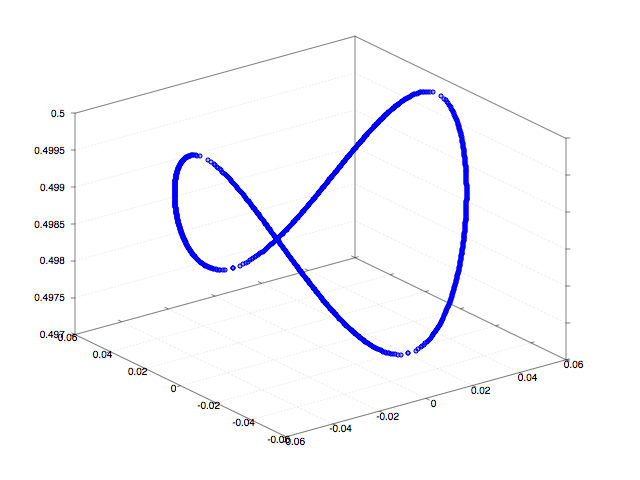
\includegraphics[width=\linewidth]{cylinder_intersection_pringle.png}
    \caption{Pringle}
    \label{fig:1b-a}
  \end{subfigure}
  %%
  \begin{subfigure}{.45\textwidth}
    \centering
      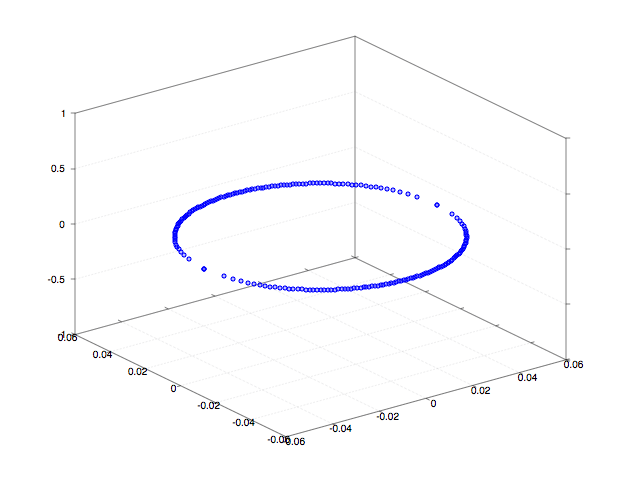
\includegraphics[width=\linewidth]{cylinder_intersection_domain.png}
    \caption{\(z\)-agnostic domain}
    \label{fig:1b-b}
  \end{subfigure}
  %%
  \caption{Intersection of Cylinders}
  \label{fig:1b}
\end{figure}

Plotting this via
\begin{verbatim}
z = sqrt(1/4 - 1/400):0.00001:sqrt(1/4);
x = sqrt(z.*z - 99/400);
y = sqrt(1/4 - z.*z);
pts1 = [x; y; z];
pts2 = [-x; y; z];
pts3 = [x; -y; z];
pts4 = [-x; -y; z];
pts = [pts1, pts2, pts3, pts4];

otherx = -sqrt(1/400):0.001:sqrt(1/400);
othery = sqrt(max(1/400 - otherx.*otherx, 0));
otherpts1 = [otherx; othery; zeros(size(otherx))];
otherpts2 = [otherx; -othery; zeros(size(otherx))];
otherpts = [otherpts1, otherpts2];

scatter3(pts(1, :), pts(2, :), pts(3, :));
figure;
scatter3(otherpts(1, :), otherpts(2, :), otherpts(3, :));
\end{verbatim}
we see in Figure~\ref{fig:1b} that the intersection is a ``pringle'' shape.

From this it's clear that points with \(z > 0.5\) (and also below
\(0.7 - \sqrt{0.0075}\), where the sphere ends) must be on the dendrite.
Also points with \(z < \sqrt{0.2475}\) must be on the ``main line''. However
points in between can be on either one. For such points, we must also know
the \(x, y\) values. If \(x^2 + y^2 > 0.05^2\), then the point must be on
the main line. If \(x^2 + y^2 < 0.05^2\), then it must be thrown away ---
this would be a part of the ``main line'' cylinder covered up by the interior
of the dendrite cylinder. If \(x^2 + y^2 = 0.05^2\) then it lies on the
dendrite. For points on the dendrite, if \(y^2 + z^2 < 0.5^2\), then we
discard the point.

Using
\begin{verbatim}
theta = 0:0.05:(2*pi);
r = 0.05;
xPoints = r * cos(theta);
yPoints = r * sin(theta);
zPoints = sqrt(0.2475):0.0001:0.505;
duplicateX = transpose(xPoints) * ones(size(zPoints));
duplicateY = transpose(yPoints) * ones(size(zPoints));
duplicateZ = ones(size(transpose(xPoints))) * zPoints;

duplicateX = reshape(duplicateX, 1, numel(duplicateX));
duplicateY = reshape(duplicateY, 1, numel(duplicateY));
duplicateZ = reshape(duplicateZ, 1, numel(duplicateZ));

cylinderPoints = [duplicateX; duplicateY; duplicateZ];
ysqPluszSq = (cylinderPoints.^2)(2, :) + (cylinderPoints.^2)(3, :);
goodIndices = (ysqPluszSq > 0.5^2);
cylinderPoints = cylinderPoints(:, goodIndices);

scatter3(cylinderPoints(1, :), cylinderPoints(2, :), cylinderPoints(3, :));
\end{verbatim}
we see in Figure~\ref{fig:1c} the shape of the dendrite at the boundary
using this rule.

We similarly crop the main line part using
\begin{verbatim}
theta = -pi/10:0.005:pi/10;
r = 0.5;
xPoints = -0.06:0.003:0.06;
yPoints = r * sin(theta);
zPoints = r * cos(theta);

duplicateX = ones(size(transpose(yPoints))) * xPoints;
duplicateY = transpose(yPoints) * ones(size(xPoints));
duplicateZ = transpose(zPoints) * ones(size(xPoints));

duplicateX = reshape(duplicateX, 1, numel(duplicateX));
duplicateY = reshape(duplicateY, 1, numel(duplicateY));
duplicateZ = reshape(duplicateZ, 1, numel(duplicateZ));

mainCylinderPoints = [duplicateX; duplicateY; duplicateZ];
xsqPlusySq = (mainCylinderPoints.^2)(1, :) + (mainCylinderPoints.^2)(2, :);
goodIndices = (xsqPlusySq > 0.05^2);
mainCylinderPoints = mainCylinderPoints(:, goodIndices);

scatter3(mainCylinderPoints(1, :), mainCylinderPoints(2, :), ...
         mainCylinderPoints(3, :));
\end{verbatim}
and produce Figure~\ref{fig:1d}.

\begin{figure}
  \centering
    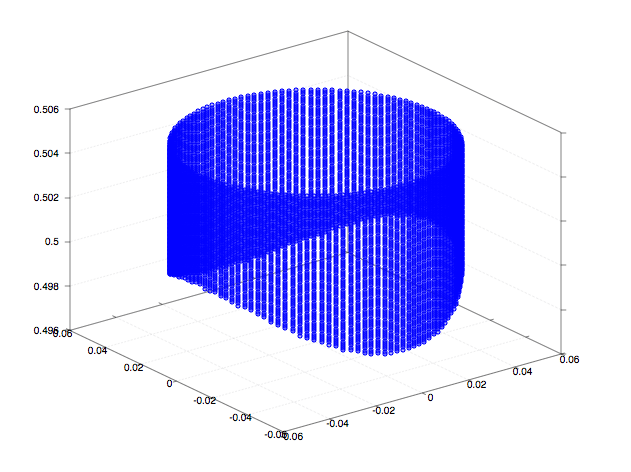
\includegraphics[scale=0.5]{top_part_dendrite.png}
  \caption{Dendrite above Main Line}
  \label{fig:1c}
\end{figure}

\begin{figure}
  \centering
    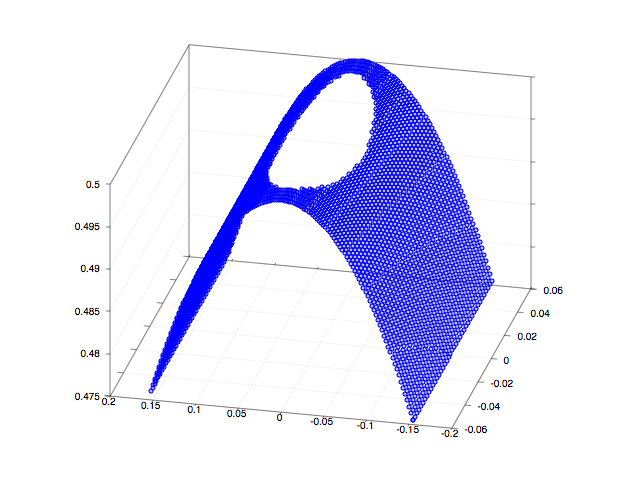
\includegraphics[scale=0.5]{cropped_main_line}
  \caption{Cropped Main Line}
  \label{fig:1d}
\end{figure}

\begin{figure}
  \centering
    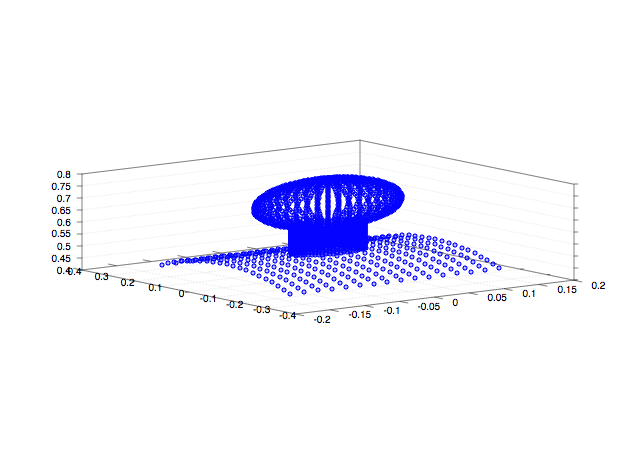
\includegraphics[scale=0.5]{whole_phenomenon.png}
  \caption{Complete Picture}
  \label{fig:1e}
\end{figure}

Using
\begin{verbatim}
theta = pi/2:0.1:pi;
phi = 0:0.15:(2*pi);
r = 0.1;

x = r * transpose(sin(theta)) * cos(phi);
x = reshape(x, 1, numel(x));

y = r * transpose(sin(theta)) * sin(phi);
y = reshape(y, 1, numel(y));

z = r * transpose(cos(theta)) * ones(size(phi));
z = 0.7 + reshape(z, 1, numel(z));

goodIndices = (z > 0.7 - sqrt(0.0075));
x = x(goodIndices);
y = y(goodIndices);
z = z(goodIndices);

spherePts = [x;y;z];

%% Do the dendrite
theta = 0:0.1:(2*pi);
r = 0.05;
xPoints = r * cos(theta);
yPoints = r * sin(theta);
zPoints = sqrt(0.2475):0.007:(0.7 - sqrt(0.0075));
duplicateX = transpose(xPoints) * ones(size(zPoints));
duplicateY = transpose(yPoints) * ones(size(zPoints));
duplicateZ = ones(size(transpose(xPoints))) * zPoints;

duplicateX = reshape(duplicateX, 1, numel(duplicateX));
duplicateY = reshape(duplicateY, 1, numel(duplicateY));
duplicateZ = reshape(duplicateZ, 1, numel(duplicateZ));

cylinderPoints = [duplicateX; duplicateY; duplicateZ];
ysqPluszSq = (cylinderPoints.^2)(2, :) + (cylinderPoints.^2)(3, :);
goodIndices = (ysqPluszSq > 0.5^2);
cylinderPoints = cylinderPoints(:, goodIndices);

%% Do the Main Line
theta = -pi/6:0.05:pi/6;
r = 0.5;
xPoints = -0.15:0.02:0.15;
yPoints = r * sin(theta);
zPoints = r * cos(theta);

duplicateX = ones(size(transpose(yPoints))) * xPoints;
duplicateY = transpose(yPoints) * ones(size(xPoints));
duplicateZ = transpose(zPoints) * ones(size(xPoints));

duplicateX = reshape(duplicateX, 1, numel(duplicateX));
duplicateY = reshape(duplicateY, 1, numel(duplicateY));
duplicateZ = reshape(duplicateZ, 1, numel(duplicateZ));

mainCylinderPoints = [duplicateX; duplicateY; duplicateZ];
xsqPlusySq = (mainCylinderPoints.^2)(1, :) + (mainCylinderPoints.^2)(2, :);
goodIndices = (xsqPlusySq > 0.05^2);
mainCylinderPoints = mainCylinderPoints(:, goodIndices);

%% Plot the whole thing
allPts = [spherePts, cylinderPoints, mainCylinderPoints];
scatter3(allPts(1, :), allPts(2, :), allPts(3, :));
axis equal;
\end{verbatim}
we are able to bring this all together as in Figure~\ref{fig:1e}.

\textbf{Moving Particles} To move we need to both move within our distinct
regions and across a change in region. To handle the move on the sphere
we use spherical coordinates with a change of basis. Typically we use
\[r, \theta, \varphi \in \left[0, \infty\right) \times \left[0, 2\pi\right)
\times \left[0, \pi\right]\]
but we will use an augmented system which forces a given point on a diameter
so that we have great circles of the full circumference in both the
\(\theta\) and \(\varphi\) direction. Using the standard spherical
coordinate  system, only points with \(\varphi = \frac{\pi}{2}\) are on
a diameter in the \(\theta\) direction. Using
\begin{align*}
x &= r \cos \left(\theta + \alpha\right) \sin \left(\varphi + \beta\right) \\
y &= r \sin \left(\theta + \alpha\right) \sin \left(\varphi + \beta\right) \\
z &= r \cos \left(\varphi + \beta\right)
\end{align*}
and consider
\[r, \theta, \varphi \in \left[0, \infty\right) \times \left[0, 2\pi\right)
\times \left[-\beta - \frac{\pi}{2}, -\beta + \frac{\pi}{2}\right]\]
XXX THIS IS WRONG AND PROBABLY GOING NOWHERE XXX

\[\left[ \begin{array}{c c}
1 & 0 \\
0 & 1
\end{array}\right]\]



\end{document}
